\documentclass[titlepage,12pt]{article}
\usepackage[UTF8]{ctex}
\usepackage{xeCJK}
\usepackage{graphicx}
\usepackage{subcaption}
\usepackage{lettrine}
\usepackage{shapepar}
\usepackage{enumitem}
\usepackage{listings}
\usepackage{geometry}
\usepackage{amsmath}
\geometry{a4paper,left=3cm,right=3cm}


\title{实验器械文档}
\begin{document}

\maketitle

\section{实验器械说明}
进入大脑的血流量主要由血泵和心脏提供,既使用脉动泵替代心脏,血液经过大脑循环后通过静脉流出。
脑脊液由另一装置产生,经过脑脊液循环被蛛网膜下腔吸收。

\section{实验器材}

Pressure sensors Series 41X, Keller AG

\subsection{心脏体外脉动循环模拟系统设计与开发研究}
颅骨CT数据导入mimics,使用灰度图像将骨与非骨分开,重建导出STL文件,最后3D打印成形。打印材料使用水溶性的聚乙烯醇(PVA)。

压力传感器选用北京星仪压阻式压力传感器,系统测量压力值小于30Kpa(即225mmHg)。图片参考论文

流量传感器选用大连博声涡轮流量传感器,量程上限$5\times10^{-6} \, \text{m}^2/\text{s}$,精度0.5级。图片参考论文
\subsection{基于模拟循环系统旋转血泵生理控制研究}
\begin{enumerate}
    \item 压力传感器:MIK-P300, MEACON, 中国;
    \item 流量计:美国 Transonic 超声波血流仪,型号 T110/H9XL;
    \item 模拟容器:有机玻璃加工,具体容积见文中各部分的详细介绍;
\end{enumerate}

\subsection{脉动流左心室辅助装置血流动力学及生理控制研究}
\begin{enumerate}
    \item 压力传感器为美国 OMEGA 公司生产的  PX409 型,测量范围±776mmHg,精度 0.6\%。
    \item 流量传感器选用  德国 SONOTEC 公司的 SONOFLOW-CO.56/120 型夹式流量计,测量范围 0L/min~12L/min,精度±2\%。
\end{enumerate}

\subsection{脉动流血泵叶轮调控关键技术研究}
\subsubsection{动脉顺应性室结构设计}
人体动脉包含大动脉以及众多的动脉分支,其本质为具有一定弹性的管道。为了模拟动脉的顺应性,忽略动脉的分布特性,将动脉系统集总化并视为一个密闭的弹性腔。
利用气体的可压缩性,将顺应性室设计成一个气液共存的密闭圆柱形容器,容器上部分为空气层,下部分为充盈的液体,如图所示。容器材料为透明亚克力,可以明显地观测气液交界面。
顺应性室底部有入口和出口两个接口,分别与动脉管道和阻尼阀相连。顺应性室顶部与气阀连接,通过调节气阀改变空气容积,进而改变空气的弹性,模拟动脉不同的顺应性值。

\begin{figure}[htbp]
    \centering
    \begin{subfigure}[b]{0.40\textwidth}
        \centering
        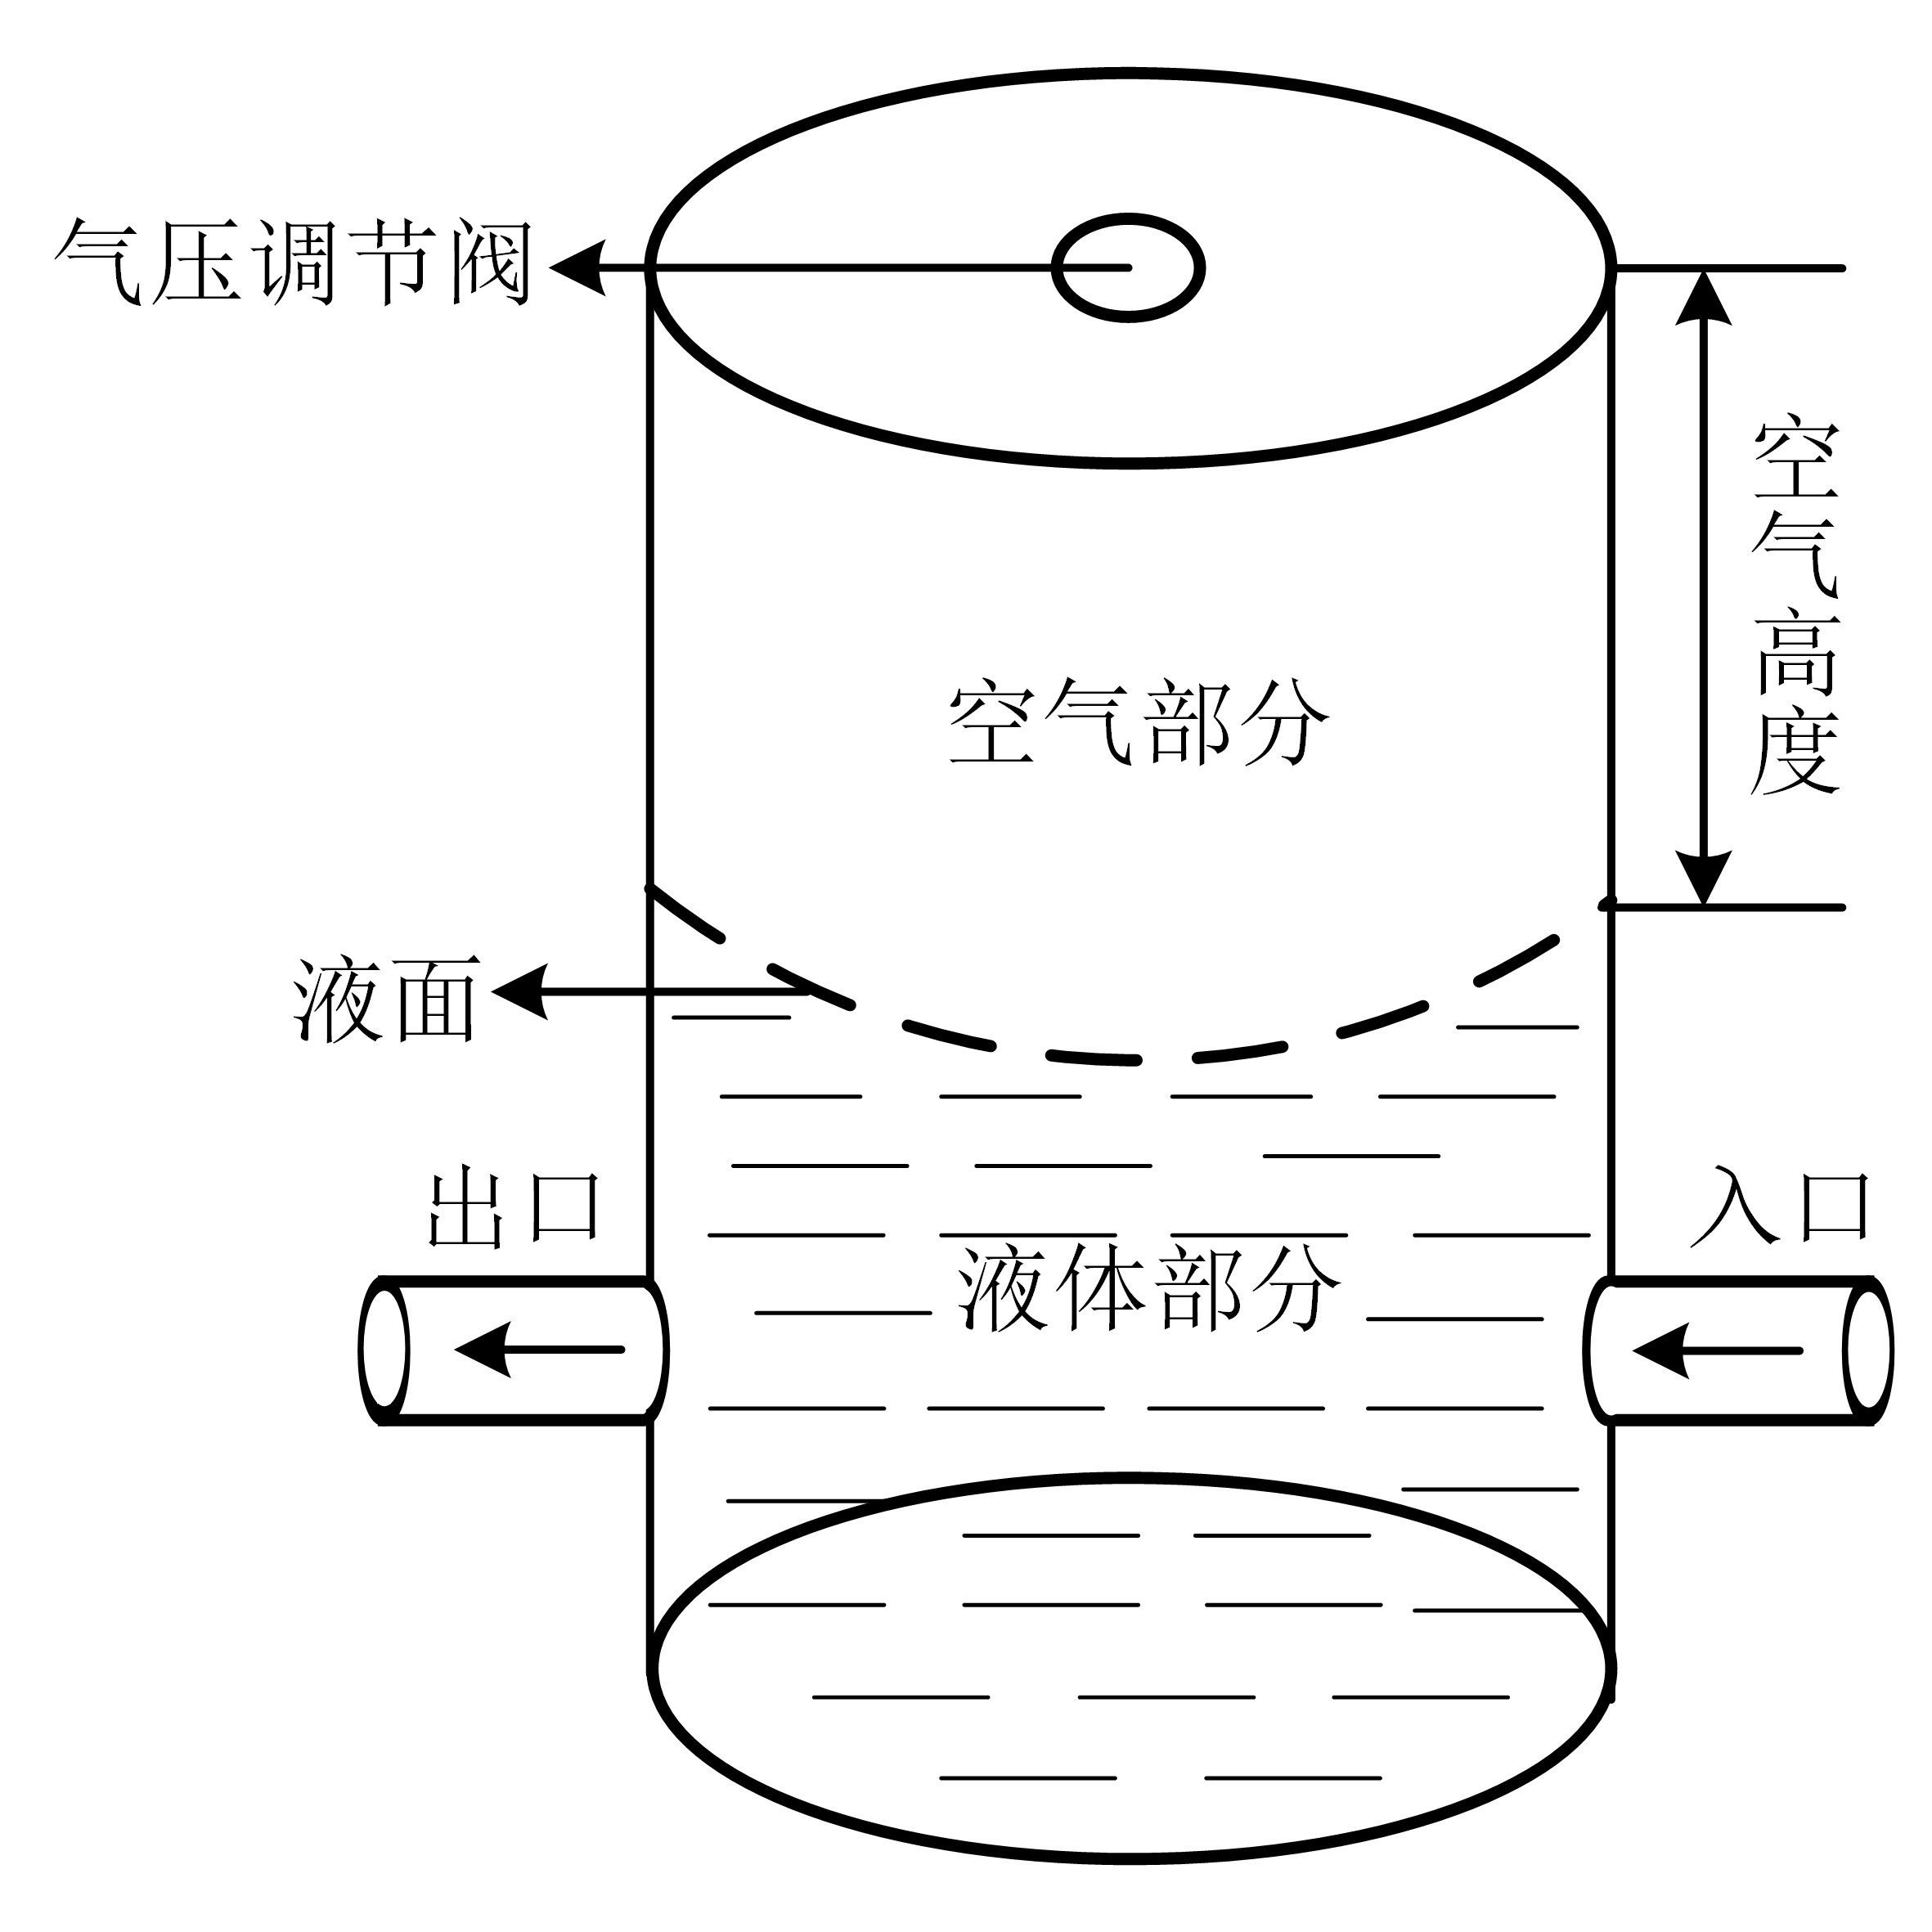
\includegraphics[width=\textwidth]{figures/顺应性示意图.png}
        \caption{顺应性示意图}
        \label{fig:compliance_diagram}
    \end{subfigure}
    \hfill
    \begin{subfigure}[b]{0.45\textwidth}
        \centering
        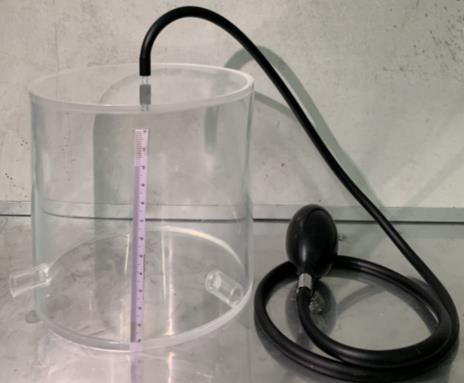
\includegraphics[width=\textwidth]{figures/顺应性实物图.png}
        \caption{顺应性实物图}
        \label{fig:compliance_real}
    \end{subfigure}
    \caption{顺应性室的示意图和实物图}
\end{figure}


\subsection{Fontan循环腔肺辅助装置的血流动力学自适应控制及生理特征评估}
\begin{enumerate}
    \item 流量传感器(Transonic Systems, Ithaca, NY,USA)
    \item 压力传感器(Millar Instruments, Houston, TX,USA)
\end{enumerate}

\end{document}